
%
%  $Description: Project Proposal for CSE 825$
%
%  $Author: Vince Fasburg, Bonnie Reiff, Josh Thomas $
%  $Date: 2015/02/09 $
%  $Revision: 1.1 $
%

\documentclass{ieee}

%------------------------------------------------------------------------- 
% 
% Use \documentclass[pagenumbers]{ieee}
%
% to produce page numbers, bottom centered, in the output. Default is 
% no page numbers for camera-ready copy.
%
%------------------------------------------------------------------------- 

\usepackage{times}
\usepackage{graphicx}

\begin{document}

\title{CSE 825: Project Proposal \\
USB Keyboard and Mouse Spoofing\\
}

\author{Vince Fasburg, Bonnie Reiff, and Josh Thomas\\
Dept of Computer Science and Engineering, Michigan State University\\
East Lansing, MI, USA\\
\{Vincent.Fasburg, Bonnie.Reiff, Josh.Thomas\}@ge.com\\
}

\maketitle
\thispagestyle{empty}

%------------------------------------------------------------------------- 
\section{Problem Definition}

Universal Serial Bus (USB) technology has become ubiquitous within our society since the turn of the twenty-first century. This type of the connection has become the standard for computer peripherals (such as keyboards, mouses, printers, external disk drives, etc.) and has also become a common method of connecting devices such as smart phones and digital cameras to computers for power supply and media transfer. It is important for this proposed project to note that all hardware attached to the computer via USB (and other protocols as well) requires an individual device driver in order to enable communication with the computer. Device drivers provide a software interface between the computer and the hardware, allowing the computer to access functions without knowing the exact details of the hardware. Typically, installation of a new device driver is the only obvious notification from a computer desktop that a USB device has been plugged into the computer \textemdash{} the operating system will not ask the user if he or she wishes to allow the device.

This project will focus on the emulation of Human Interface Devices (HIDs), specifically a keyboard and a mouse, through the use of a programmable microcontroller. More will be explained about how this emulation is possible in the ``Approach" section of this proposal. The future findings of this project can possibly be extended to other USB-connected devices as well, as demonstrated by Karsten Nohl and Jakob Lell at the Black Hat USA Conference in 2014 when they reprogrammed a USB flash memory device to emulate HIDs \cite{nohl}. Through use of keyboard commands and shell scripting, as well as mouse automation to interact with GUI elements, the microcontroller can essentially perform any task available for the current privilege level of the system within seconds, unbeknownst to to user. In order to launch these attacks, the malicious hacker need only plug in the USB device for a short amount of time. For example, this can be done if a user leaves a computer unlocked. Alternatively, the malicious hacker may get the user to plug the device in themselves, as users tend to have a trust that USB devices will not run any programs on their computers without their consent.

With this background in mind, the proposed project has the goal of answering three questions through both research and implementation:

\begin{enumerate}
\item \textit{What is the extent of attacks the can be performed using USB-HID emulation?}

Initial research for this project has shown attacks on Windows and Apple PC operating systems that include actions such as setting up a reverse shell and changing the Domain Name System (DNS) server (see the ``Previous Work" section for full explanations and citations). The proposed project will explore how these attacks, as well as many others, can be implemented for a  Linux operating system using a programmable USB microcontroller. This suite of attacks will be also be used during the second portion of the project, in which defenses against these attacks will be explored.

\item \textit{What are the existing defenses against HID emulation attacks?}

This question is essentially answered in this project proposal in the ``Previous Work" section, but is included in the Problem Definition because it will be important to final report for the project. The goal of the project is for the team to design defenses against USB-HID emulation attacks, and thus it is important to know this information  in order to compare the approaches that have been taken on features such as feasibility, strength, etc.

\item \textit{Can drivers be designed for USB mouses and keyboards to defend against HID emulation attacks?}

This final question is the most essential and significant to the project as it will require designing and implementing a new concept for USB-HID devices, as well imagining the ways in which the newly implemented defenses can be weakened. The overall goal is to implement drivers for USB mouses and keyboards that have the ability to distinguish between emulated (malicious) devices and human-controlled devices. As will be explained in the following sections, the team has some initial ideas on how this can be done, but there are weaknesses to those ideas that will need to be overcome.

\end{enumerate}

%------------------------------------------------------------------------- 
\section{Approach}

The team is proposing a two part project which includes exploiting a few weaknesses in a computer system by creating a suite of attacks, then offering a solution to those weaknesses by developing one or more drivers to prevent future attacks. This section will describe the approach for each part of the project as well as the equipment the team will need.

For the first part of the project, the team will program a Teensy microcontroller, shown in Figure~\ref{fig:Teensy}, to run a suite of attacks on a Linux operating system. The main idea would be to emulate a USB keyboard and mouse with the Teensy so that the computer's Linux operating system will recognize the Teensy as a ``safe" device. This is easily achievable after installing Arduino and Teensyduino software on the computer being used to program the Teensy using the development environment option to use a board the emulates a USB keyboard and mouse. Once the operating system believes that the Teensy is a safe device, the program can send keyboard or mouse commands to the operating system. The operating system should not notice anything different about these commands as compared to the commands coming from an actual keyboard or mouse. A broad range of attacks will be created, including some which would require administrative privileges.

\begin{figure}[H]
   \center{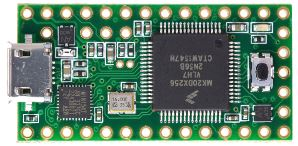
\includegraphics{Pictures/Teensy}}
   \caption{Teensy Microcontroller}
   \label{fig:Teensy}
\end{figure}

This class of attacks is potentially very dangerous because once the program has the ability to the use the keyboard and mouse, a Linux terminal can be opened to do almost anything to the system, for example, ``rm -rf *'' which recursively wipes all of the files from the current directory on the drive. The program could easily run without the user being aware since a terminal window could be opened up and immediately minimized while the program is still running. After only a few seconds, the program could be finished running and have the terminal window closed all before the user realizes anything is wrong.

For the second part of the project, the team will work on preventing the attacks that were created in the first part by developing Linux drivers to authenticate the USB device before any attached keyboard or mouse is allowed to be used normally. Some preliminary ideas include using a series of Turing tests to determine if the input device is being used by a computer or a human. Essentially, a Turing test is a test of a machine's ability to exhibit human behavior indistinguishable of that of a human \cite{wiki}.

To test a keyboard device, a random text captcha, as shown in  Figure~\ref{fig:Captcha}, could be used. The program installed on the Teensy will not know what the random captcha text is going to be, so a human user is required to type in the letters by hand before the keyboard is allowed to be used. In addition, a mouse could be verified by requiring a user to follow a randomly generated pattern on the screen or point and click to something in a random location on the screen to verify that a human is the one sending the commands as a mouse. If any of these tests fail, no other input is allowed from the device until the captcha or pattern is complete.

\begin{figure}[H]
   \center{
\includegraphics{Pictures/captcha}}
   \caption{Captcha Example}
   \label{fig:Captcha}
\end{figure}

%------------------------------------------------------------------------- 
\section{Previous Work}

The Teensy microcontroller has been used for many purposes, including mounting many different HID based attacks on various systems that accept input from USB human interface devices. An excellent resource that demonstrates the need for HID authentication is the website of Samy Kamkar \cite{samy}, in which the author shows an attack he calls ``USBDriveby''. The USBDriveby attack uses a Teensy microcontroller, emulating a keyboard and a mouse simultaneously,  to create a permanent connection to a remote server that is controlled by the attacker.  This connection will be re-established regularly so that the attacker can issue commands to the machine at any point in the future, including after the microcontroller has been disconnected from the victim's machine.

This example of an emulated HID-based attack serves to show the severity with which a system can be compromised when a malicious USB device is connected for even a short time, and without requiring an administrator password. Although the USBDriveby attack was created for the Apple OSX operating system, similar attacks may be possible on any other system that accepts USB inputs. The list of potential attacks is very large, including attacks with various effects to the victim, and ranging from very simple to very complex in implementation.

Although some attempts have been made to develop a mechanism for the authentication of USB devices, much less attention has been paid to the authentication of USB human interface devices. In a paper \cite{wang} proposing an extension to a USB driver to authenticate USB connections, the proposed 2-way authentication mechanism specifically excludes ``non-programmable devices'' such as a USB keyboard. This seems sensible, but leaves a system vulnerable to programmed attacks hiding inside a ``non-programmable device''.

Among the literature dealing with USB device security, some papers such as ``Plug \& Prey: Malicious USB Devices'' come closer to a solution regarding malicious HIDs. The paper describes how, on Windows, you can use registry changes to prevent USB devices from being installed. However, this would prevent legitimate HIDs from being installed also, unless a whitelist of vendor IDs and product IDs is used to allow certain devices. However, these properties can be spoofed, so the Teensy device may appear to be a whitelisted device.

The final suggestion in this paper is to apply settings to allow administrators to override the policy preventing the installation of a HID. This technique would run into problems if the device in question were the first HID to be connected to the machine, as the user would have no way to allow the installation. Furthermore, it requires administrative privileges to plug in a keyboard or mouse. The mechanism to disable installing USB devices is very different for Linux system, but the results and limitations are roughly the same.

A novel approach to USB authentication specifically for HIDs was proposed by Barbhuiya et al. \cite{barbhuiya}, which relies on either continuous or periodic authentication based on keystroke dynamics, including metrics such as the speed of typing, and the relative times of presses and releases of the keys. This method uses a stored profile of typing behaviors from the authentic user to determine whether the keystroke dynamics exhibited by the inputs are a match to the known patterns. If the keystroke dynamics are determined not to match the stored profile, the input will not be processed.

The keyboard dynamics approach to preventing emulated HID attacks would likely succeed most of the time. However, there are some significant drawbacks in this type of technique from a usability standpoint, stemming from both false positive and false negative authentication. Consider that an attack from a malicious device may be extremely short, and thus more likely to be unintentionally allowed through the authentication (consider the command ``rm -rf *''). If the malicious device were programmed to enter input in a human seeming way (perhaps emulating keyboard dynamics of an average human), there is a significant chance that small amounts of inputs would be accepted \cite{shahzad}. Furthermore, a user using a computer equipped with keystroke dynamics based authentication may reject input from a legitimate user if keystroke patterns change do to any variation in the environment or the user. Lastly, the principles of keyboard dynamics cannot easily be generalized to include authentication for a mouse as well as a keyboard.

Finally, at the 2014 Las Vegas Black Hat Security Conference, Karsten Nohl and Jakob Lell presented several USB based attacks that they collectively referred to as BadUSB \cite{nohl}. Among the attacks described is the malicious emulation of a HID. This section of the presentation describes how an emulated keyboard could be used to steal the administrative password on a Linux system, then allowing the device to perform other actions using the sudo command. The only defenses proposed in this presentation that would be suitable against an emulated keyboard or mouse were to block USB devices entirely, or by using a blacklist or whitelist of device types. As stated previously, such defenses can easily be overcome by spoofing a legitimate device ID.

%------------------------------------------------------------------------- 

\appendix 

%\newpage% -- remove this comment if we want the Appendix and References on a new page

\section{Appendix: Team Contributions}

All team members contributed equally to the research of possible ideas for the project topic. For the project proposal document, the work was divided as follows, with each team member being assigned to one section:

\begin{enumerate}
\item Problem Definition - Bonnie Reiff
\item Approach - Josh Thomas
\item Previous Work - Vince Fasburg
\item LaTeX - Josh Thomas and Bonnie Reiff
\item Setup github Repository - Vince Fasburg
\end{enumerate}

All team members were responsible for final read through and editing of the document.


%------------------------------------------------------------------------- 

\bibliographystyle{ieee}
\bibliography{bibfile}

\end{document}

